\documentclass[a4paper,12pt,twoside]{article}
\usepackage[latin1,utf8]{inputenc}
\usepackage[spanish]{babel}
\usepackage[T1]{fontenc}
\usepackage[usenames]{color}
\usepackage{amsmath}
\usepackage{amssymb}
\usepackage{setspace}
\usepackage{booktabs}
\usepackage{pifont}
\usepackage{hyperref}
\usepackage[spanish]{babelbib}
\usepackage[nottoc,numbib]{tocbibind}
\usepackage{enumitem}
\usepackage{eurosym}
\usepackage{epsfig}
\usepackage{cite}
\usepackage{textcomp}
\usepackage[a4paper,bindingoffset=0.cm,%
            left=2.5cm,right=2.5cm,top=3.5cm,bottom=2.5cm,]{geometry}
%\usepackage[style=numeric,maxnames=3]{biblatex}
%\documentstyle[12pt]{article}
%\setlength{\textheight}{27.2cm}
%\setlength{\textwidth}{18.5cm}
%\setlength{\oddsidemargin}{2.5cm}
%\setlength{\evensidemargin}{2.5cm}
%\setlength{\topmargin}{2.5cm}

%\setlength{\parindent}{0pt}
%\addtolength{\topmargin}{-1.5cm}
%\addtolength{\oddsidemargin}{-1.8cm}
%\addtolength{\evensidemargin}{-1.cm}

%%%%%%% espacio entre lineas %%%%%%%%
%\renewcommand{\baselinestretch}{1.25}
%%%%%%%%punto decimal%%%%%%%%%%%%%%%%


%\def\ket#1{|#1\rangle}
%\def\bra#1{\langle#1|}
%\def\scal#1#2{\langle#1|#2\rangle}
%\def\matr#1#2#3{\langle#1|#2|#3\rangle}
%\def\bino#1#2{\left(\begin{array}{c}#1\\#2\end{array}\right)}
%\def\ave#1{\langle #1\rangle}
%\def\dis#1{\langle\langle #1\rangle\rangle}
%\def\uvo#1{\lq #1\rq\ }
%\def\uuvo#1{\lq\lq #1\rq\rq\ }
%\def\ave#1{\langle#1\rangle}
%\newcommand{\field}[1]{\mathbb{#1}}
%\newcommand{\ra}{\rangle}
%\newcommand{\la}{\langle}
%\newcommand{\rp}{\right)}
%\newcommand{\lp}{\left(}
%\newcommand{\rc}{\right]}
%\newcommand{\lc}{\left[}
%\newcommand{\arctanh}{\mbox{arctanh\hspace{0.05cm}}}
%\newcommand{\obeta}{\overline{\beta}}
%\newcommand{\onu}{\overline{\nu}}

%\usepackage{titlesec}


%\titleformat{\chapter}[hang]{\bf\huge}{\thechapter}{2pc}{}

\usepackage{fancyhdr}
 
\pagestyle{fancy}
\fancyhf{}
\fancyhead[RE,LO]{\underline{\nouppercase{\rightmark}}}
\fancyhead[LE,RO]{\thepage}
\renewcommand{\headrulewidth}{0pt}
%\rfoot{Page }
 
%\onehalfspacing
\spacing{1.5}

\addto\captionsspanish{\renewcommand{\tablename}{Tabla}}

\begin{document}

%\renewcommand{\refname}{Bibliografía}

\title{\textbf{Proyecto: Planteamientos docentes e investigadores}}
\author{Mario G\'omez Ramos}
\maketitle
%\begin{figure}
%\centering
%\includegraphics[height=3cm]{us.pdf}
%\end{figure}

\thispagestyle{empty}
\newpage
\thispagestyle{empty}  

~ \\


\newpage
\section*{Pre\'ambulo}

El presente documento sigue las indicaciones del BOJA Número 88 de 12 de mayo de 2025. Se establece la presentación de un proyecto con los planteamientos docentes e investigadores del candidato. Se debe respetar la extensión máxima de 50 páginas en A4 con letra de 12 puntos de cuerpo, con espaciado interlineal de 1.5 y márgenes de 2.5 cm.

Atendiendo a estas indicaciones el documento se divide en los siguientes apartados:

\begin{itemize}
\item Introducción
\item Planteamientos docentes
\item Planteamientos investigadores
\end{itemize}

\vfill


Mario G\'omez Ramos

En Sevilla, a \today.

~ \\

~ \\

~ \\


\newpage

~ \\
%
%
\newpage

\tableofcontents
\newpage

~ \\




\section{Introducci\'on}
\label{intro}

El presente documento desarrolla los planteamientos docentes e investigadores relativos al desempeño como Profesor Permanente Laboral dentro del sistema universitario. Naturalmente, es necesario que estos planteamientos se ajusten a la concepción actual de la Universidad y busquen la consecución de sus objetivos y funciones, por lo que es conveniente analizar cuáles son estos objetivos y funciones para una universidad moderna.

La universidad de Bolonia, fundada en 1088, se considera la primera universidad del mundo, al ser la primera institución con las siguientes características:

\begin{itemize}
\item Era capaz de expedir titulaciones académicas de alto nivel.
\item Utilizó explícitamente la palabra \textit{universitas}, de \textit{niversitās magistrōrum et scholārium} (comunidad de profesores y académicos), en su fundación.
\item Era formalmente independiente de la educación eclesiástica.
\item Ofrecía estudios seculares, como gramática, lógica o derecho.
\end{itemize}

Si bien la Universidad de Bolonia, y otras fundadas en el periodo medieval, como las Universidades de París (1150), Oxford (1096) o Salamanca (1218), presentan características asociadas actualmente con las instituciones universitarias (como la libertad de cátedra), su concepción y funciones eran significativamente distintas de las de una universidad actual. Por ejemplo, la investigación, ahora íntimamente ligada al entorno universitario, tuvo que esperar a 1794 para su primera vinculación oficial a la universidad, con la creación de la primera cátedra de investigación científica por la Universidad de Cambridge.

Por lo tanto, para una concepción clara de la misión de la universidad es necesario centrarse en visiones más recientes. Por ejemplo, para Ortega y Gasset, en su trabajo \textit{Misión de la Universidad}\cite{ortega_gasset}, las funciones de la universidad son las siguientes:

\begin{itemize}
\item Ser transmisora de cultura y de la realidad de una época
\item Formar futuros profesionales y prepararlos para esta labor
\item Investigar y formar a los estudiantes en la ciencia
\end{itemize}

Por otro lado, la UNESCO, en su \textit{Declaración Mundial sobre la Educación Superior en el siglo XXI} \cite{unesco}, expande las funciones de la universidad:

\begin{itemize}
\item Función de educar, formar y realizar investigaciones
\begin{itemize}
\item Formar diplomados altamente cualificados y ciudadanos responsables.
\item Constituir un espacio abierto para la formación superior que propicie el
aprendizaje permanente.
\item Promover, generar y difundir conocimientos por medio de la investigación.
\item Contribuir a comprender, interpretar, preservar, reforzar, fomentar y difundir
las culturas nacionales y regionales, internacionales e históricas.
\item Contribuir a proteger y consolidar los valores de la sociedad.
\item Contribuir al desarrollo y la mejora de la educación en todos los niveles.
\end{itemize}
\item Función ética, autonomía, responsabilidad y prospectiva
\begin{itemize}
\item Poder opinar sobre los problemas éticos, culturales y sociales, con total
autonomía y plena responsabilidad.
\item Reforzar sus funciones críticas y progresistas.
\item Utilizar su capacidad intelectual y prestigio moral para defender y difundir
activamente valores universalmente aceptados como la paz, la justicia, la libertad, la igualdad y la solidaridad.
\item Disfrutar plenamente de su libertad académica y autonomía siendo al mismo tiempo
plenamente responsable para con la sociedad.
\item Aportar su contribución a la definición y tratamiento de los problemas que
afectan al bienestar de las comunidades, las naciones y la sociedad mundial.
\end{itemize}
\end{itemize}

Más reciente es el \textit{Comunicado de la Conferencia de Ministros de Educación Europeos} \cite{Com2009}, donde se reconocen como misiones de la universidad:

\begin{itemize}
\item  Preparar a los alumnos
para la vida como ciudadanos activos en una sociedad democrática
\item Preparar a los alumnos para su carrera profesional futura y permitir su desarrollo personal
\item Crear y mantener una
amplia y avanzada base de conocimiento
\item Estimular la investigación y la innovación
\end{itemize}

A partir de todos estos documentos, se hace patente que diversos actores e instituciones presentan distintas visiones sobre la función de la universidad en la sociedad, si bien hay dos pilares que surgen consistentemente, asociados con la generación y transmisión de conocimiento por parte de la comunidad universitaria: investigación y docencia. Son estas dos funciones del personal universitario las que se discutirán en las siguientes secciones.

\section{Planteamientos Docentes \label{sec:docente}}

En esta sección se presentan los planteamientos docentes del candidato. Se presenta el contexto normativo e institucional de las legislaciones relevantes y se presenta la Universidad de Sevilla como institución particular en la que se realizará la labor docente, como contexto sobre el que se introducen los planteamientos, que, aunque se presentan de manera general, en los casos en los que sea necesario se particularizarán a la asignatura de Física Nuclear y de Partículas. 

\subsection{Marco normativo e institucional}

\subsubsection{Espacio Europeo de la Enseñanza Superior}

El Espacio Europeo de la Enseñanza Superior (EEES) surge en un esfuerzo por armonizar la educación superior en distintos países de la Unión Europea y mejorar su competitividad. Siguiendo los principios fundamentales expuestos en la \textit{Magna Charta Universitatum} \cite{magna_charta}, firmada en Bolonia en 1988, los objetivos del EEES son los siguientes, recogidos en la declaración de Bolonia de 1999 \cite{bolonia}:

\begin{itemize}
\item Adopción de un sistema de títulos fácilmente comprensibles y comparables.
\item Adopción de un sistema basado esencialmente en dos ciclos principales.
\item Puesta a punto de un sistema de créditos, como el sistema ECTS, para promover una mayor movilidad entre los estudiantes.
\item Promoción de la movilidad mediante la eliminación de los obstáculos al ejercicio efectivo del derecho a la libre circulación.
\item Promoción de la cooperación europea en materia de aseguramiento de la calidad.
\item Promoción de la necesaria dimensión europea en la enseñanza superior.
\end{itemize}

Esta declaración de Bolonia fue firmada por los ministros de 29 países y actualmente son 49 los países que forman parte del EEES, con reuniones periódicas, la última de las cuales tuvo lugar en Tirana (Albania) en 2024. Pilares fundamentales del EEES son los créditos ECTS, el sistema de dos ciclos (grado y posgrado) y el cambio en la metodología docente, que se describen a continuación:

\textbf{El sistema de créditos ECTS (Sistema Europeo de Transferencia de Créditos)} 

Para favorecer la movilidad de los estudiantes entre distintos centros del EEES y la convalidación de los estudios realizados en ellos, es necesario definir una unidad de medida común para el trabajo desempeñado por el estudiante en base a la cual se pueda considerar si el estudiante cumple los requisitos necesarios para la concesión del título correspondiente. Dentro del EEES, esta unidad de trabajo se corresponde con el crédito ECTS, de las iniciales en inglés de Sistema Europeo de Transferencia de Créditos. Debido a que las competencias de educación corresponden a los estados, distintos estados dentro del EEES pueden presentar distintos requisitos sobre el trabajo que corresponde a 1 ECTS. Dado que este proyecto se corresponde a una universidad española, se presentan los criterios recogidos por la legislación española, introducido por el Real Decreto 1125/2003 de 5 de septiembre \cite{dec_ects}. De acuerdo a este decreto, un crédito debe corresponder a 25-30 horas del trabajo de un alumno, incluyendo trabajo dentro y fuera del aula, con un número de créditos total para un curso académico de 60 a repartir en unas 36-40 semanas anuales, resultando en una dedicación de unas 37.5 horas, es decir, a tiempo completo.

Dado que el trabajo personal del alumno para cumplir con los objetivos de una asignatura dependerá de las circunstancias y capacidades de dicho alumno, esta relación entre horas de trabajo y número de créditos ECTS debe tomarse como una primera aproximación, siendo parte de la labor docente ajustar los objetivos de las distintas asignaturas para que un alumno medio pueda alcanzarlos con una dedicación próxima a la teórica. Es destacable que a la hora de asignar créditos de docencia al profesorado no es habitual tomar el trabajo personal del docente en consideración, de manera que créditos que corresponden a cargas de trabajo significativas para el docente, como aquellos asociados a trabajos fin de curso, suelen infrarrepresentar el esfuerzo por parte del docente. En este sentido, sería deseable una mejora en los sistemas de asignación de créditos al profesorado.

\textbf{Ciclos de grado y posgrado}

El sistema del EEES presenta la reestructuación de la educación superior en cursos de grado y posgrado, los primeros habilitando al estudiante a acceder al mercado laboral y a los estudios de posgrado, y los segundos correspondiendo a una mayor especialización. Dentro del sistema español, el estudio de posgrado se corresponde a los estudios de máster. El acceso a los estudios de doctorado requiere la compleción de 300 ECTS entre estudios de grado y máster, siendo indispensable el curso de un máster previo al doctorado. Estos estudios están actualmente regulados por el Real Decreto 822/2021, de 28 de septiembre \cite{dec_master}.

En lo que corresponde al grado, son estudios que prestan \textit{enseñanzas básicas y de formación general, en una o varias disciplinas, orientadas
también a la preparación para el ejercicio de actividades de carácter profesional} y la gran mayoría de los estudios corresponden a 240 créditos ECTS (4 años), aunque pueden ser de 180 ECTS si las universidades arbitran mecanismos para complementar el número de créditos hasta 240 a través de titulaciones de máster, y pueden ser superiores en casos especiales, i.e. el grado en Medicina, cuyos créditos totales son 360.

Los estudios de máster buscan \textit{la adquisición por el estudiante de una formación avanzada, de carácter
especializado o multidisciplinar, orientada a la especialización académica o profesional, o
bien a promover la iniciación en tareas investigadoras} y pueden corresponderse a 60, 90 ó 120 ECTS.

Dentro de la legislación vigente, tanto los estudios de grado como de máster deben incluir la elaboración de al menos un trabajo obligatorio dentro de la titulación. Para el caso del grado se establece un trabajo fin de grado (TFG) correspondiente a un mínimo de
6 créditos y un máximo del 12,5 por ciento del total de los créditos del título. En el caso
del máster se define un trabajo fin de Máster (TFM) con una duración de entre 6
y 30 créditos.

Es notable que, pese al objetivo integrador del sistema EEES, gran parte de los países pertenecientes favorecen estudios de grado de 180 ECTS con estudios de posgrado de 120 ECTS para alcanzar los 300 necesarios para un doctorado, lo cual dificulta la armonización y convalidación de sus estudios con sistemas como el español, donde la distribución es de 240/60.

\textbf{Cambio en la metodología docente}

Como atestigua la introducción del ECTS, en el EEES los objetivos del sistema educativo se estructuran en base al trabajo y el desarrollo del alumno y sus capacidades. Dentro de la idea de una educación continua para los ciudadanos, subyacente a la declaración de Bolonia,  las competencias desarrolladas por el alumno toman un lugar prioritario sobre los contenidos, que pueden evolucionar y cambiar en el tiempo. Estas competencias se clasifican en:

\begin{itemize}
\item Competencias genéricas o transversales: aquellas globales que se desarrollan durante la formación universitaria, i.e., resolución autónoma de problemas, trabajo en equipo, comunicación oral.
\item Competecias específicas: aquellas vinculadas a áreas y capacidades
concretas de cada titulación.
\end{itemize} 

Los planes de estudio de titulaciones y asignaturas, además de la evaluación de la consecución de sus objetivos, deben realizarse con el desarrollo de estas competencias por parte del alumno en mente.

\subsection{Las Universidades en España y Andalucía}

En el artículo 27 de la Constitución Española se estipula que:

\begin{enumerate}
\item[1.] Todos tienen el derecho a la educación. Se reconoce la libertad de enseñanza.
\item[2.] La educación tendrá por objeto el pleno desarrollo de la personalidad humana en el respeto a los principios democráticos de convivencia y a los derechos y libertades fundamentales.
\item[10.] Se reconoce la autonomía de las Universidades, en los términos que la ley establezca.
\end{enumerate}

Aun con estas directrices, la competencia en materia de Educación no se indica como exclusiva del Estado, por lo que de acuerdo con el artículo 147, punto 3 de la Constitución, estas competencias pueden ser recibidas por las Comunidades Autónomas, si así lo recogen sus Estatutos. En el caso de Andalucía, efectivamente, el Estatuto de Autonomía, en su artículo 53 reconoce la competencia exclusiva de la Comunidad Autónoma sobre varios puntos asociados al sistema universitario, como la creación y autorización de universidades, programación y coordinación de sistema universitario o la regulación del acceso a las universidades y del profesorado docente investigador, todo esto sin perjuicio de la autonomía universitaria. Esta implicación tanto del Estado como de las Comunidades Autónomas en el sistema universitario, implica que este está sometido tanto a legislaciones estatales como autonómicas, además de los estatutos propios de las distintas universidades.

\subsubsection{Ley Orgánica del Sistema Universitario (LOSU)}

La ley estatal vigente que regula el sistema universitario es la Ley Orgánica del Sistema Universitario (LOSU) \cite{losu}, publicada en el BOE 70, del 23 de Marzo de 2023. Los cambios introducidos en esta ley más relevantes para la la convocatoria de esta plaza son la reducción de la temporalidad en los cuerpos docente e investigador de las universidades, imponiendo un límite del 8\% de profesorado temporal como máximo, afectando principalmente a las figuras de Profesor Asociado y Profesor Ayudante Doctor, y la modificación de las figuras docentes estables, desapareciendo la figura de Profesor Contratado Doctor y creándose la de Profesor Permanente Laboral, correspondiente a este concurso. También es notable el compromiso por incrementar el presupuesto asociado a la investigación, hasta el 1\% del PIB nacional.

\subsubsection{Ley Andaluza de Universidades (LAU)}

A nivel autonómico andaluz, la normativa vigente que cubre las universidades es la Ley Andaluza de Universidades (LAU) de 2003, desarrollada en el contexto de la Ley Orgánica de Universidades (LOU, actualmente sustituida por la LOSU). La LAU fue modificada en 2011 y su texto refundido fue publicado en 2013 \cite{lau}. Dentro de esta Ley se crea un organismo andaluz para potenciar y evaluar la calidad de la educación superior: la Agencia Andaluza de Evaluación de la calidad y la acreditación universitaria (AGAE). Este cuerpo fue reconvertido a la Dirección de Evaluación y Acreditación (DEVA), con registro en el Registro Europeo de Agencias de Calidad (EQAR) en 2014, y una vez más a la actual Agencia para la Calidad Científica y Universitaria de Andalucía (ACCUA), con registro en EQAR en 2024. Entre los objetivos de ACCUA se encuentran evaluar y acreditar a las Universidades, al profesorado y las actividades de formación e investigación, y, junto con la Agencia Nacional de Evaluación de la Calidad y Acreditación (ANECA), puede emitir acreditaciones para la figura de Profesor Permanente Laboral.

Debido al nuevo entorno legal introducido por la LOSU, la junta de Andalucía esta tramitando una nueva ley de universidades, la Ley Universitaria para Andalucía (LUPA), cuyo anteproyecto fue publicado el 3 de octubre de 2024 \cite{lupa}, entre cuyas reformas destacables se halla la restitución de la figura Profesor Contratado Doctor.

\subsection{La Universidad de Sevilla}

La Universidad de Sevilla, fundada en 1505, es la tercera de España en número de alumnos, por detrás de la UNED y la Universidad Complutense de Madrid \cite{cifras}, con $\sim$71000 alumnos matriculados, $\sim$4500 profesores y una oferta de 89 grados, 117 máster y 32 programas de doctorado en el curso 2023-2024 y está compuesta por 32 centros y 134 departamentos \cite{us}. La Universidad de Sevilla presenta buenas posiciones en rankings internacionales como el Academic Ranking of World Universities o ránking de Shanghai (485), el QS World University Ranking (462) o el NTU Ranking (447) \cite{us}.

Además de por las normativas estatales y autonómicas, la Universidad de Sevilla se rige por estatutos propios, cuya última versión ha sido publicada en el BOE el 20 de mayo de 2025 \cite{estatutos}. En el artículo 14 de dichos estatutos se establece la estructura académica de la Universidad de Sevilla, integrada por:

\begin{enumerate}[label=\alph*)]
\item Centros: facultades y escuelas. Asimismo, tendrán la consideración de centros la Escuela Internacional de Doctorado, la Escuela Internacional de Posgrado y el Centro de Formación Permanente.
\item Departamentos.
\item Institutos universitarios de investigación.
\item Centros mixtos e instalaciones científicas.
\item Otros centros y estructuras que se creen para el desarrollo de las funciones de la Universidad.
\end{enumerate}

Dado que la plaza asociada al presente concurso está asociada al Departamento de Física Atómica, Molecular y Nuclear de la Facultad de Física de la Universidad de Sevilla, los siguientes apartados corresponden a dicho centro y departamento.

\subsubsection{Facultad de Física}

En la facultad de Física se imparten las siguientes titulaciones de grado:
\begin{itemize}
\item Grado en Física
\item Grado en Ingeniería de Materiales
\item Doble Grado en Física y Matemáticas (en conjunto con la Facultad de Matemáticas)
\item Doble Grado en Física e Ingeniería de Materiales
\item Doble Grado en Química e Ingeniería de Materiales (en conjunto con la Facultad de Química)
\end{itemize} 

Las titulaciones de máster impartidas son:
\begin{itemize}
\item Máster Universitario en Microelectrónica: Diseño y Aplicaciones de Sistemas Micro/Nanométricos
\item Máster Inter-universitario en Física Nuclear (junto con la Universidad Complutense de Madrid, la Universidad Autónoma de Madrid, la Universidad de Barcelona, la Universidad de Granada, y la Universidad de Salamanca) 
\item Máster Universitario en Tecnologías Físicas para la Medicina y la Biología.
\end{itemize} 

Todos los departamento de la Facultad de Física pertenecen al programa de doctorado de Ciencias y Tecnologías Físicas.

De acuerdo con los Estatutos de la Universidad de Sevilla, es función de la facultad la elaboración de los planes de estudios de las titulaciones impartidas. Además también debe coordinar y supervisar la actividad docente de sus departamentos, que, en el caso de la Facultad de Física son 3:

\begin{itemize}
\item Departamento de Electrónica y Electromagnetismo
\item Departamento de Física Atómica, Molecular y Nuclear
\item Departamento de Física de la Materia Condensada
\end{itemize}

\subsubsection{Departamento de Física Atómica, Molecular y Nuclear}

Al Departamento de Física Atómica, Molecular y Nuclear se encuentran en la actualidad (2025) asociados 76 docentes e investigadores entre personal permanente, personal temporal, contratados predoctorales e investigadores eméritos y honorarios. Este personal se distribuye en tres áreas de conocimiento (si bien la LOSU propone una distribución por ámbitos de conocimiento, esta distribución aún no se ha materializado):

\begin{itemize}
\item Astronomía y Astrofísica
\item Física Atómica, Molecular y Nuclear
\item Física Teórica
\end{itemize}

De estas tres áreas, tanto el perfil docente como el investigador asociados a la plaza correspondiente a este concurso cuadran dentro del ámbito y las asignaturas asignadas al área de Física Atómica, Molecular y Nuclear, por lo tanto, se procede a dar información sobre esta área.

Las asignaturas obligatorias asignadas a nivel de grado al área de Física Atómica, Molecular y Nuclear son las siguientes:

\begin{itemize}
\item Física Cuántica (Grado en Física y Dobles Grados asociados)
\item Física Nuclear y de Partículas (Grado en Física y Dobles Grados asociados)
\item Técnicas Experimentales II (Grado en Física y Dobles Grados asociados)
\item Física I (Grado en Ingeniería de Materiales)
\item Física (Grado en Óptica y Optometría y Dobles Grados asociados)
\end{itemize}

A nivel de máster, el área de conocimiento tiene adscritas asignaturas del Máster Interuniversitario en Física Nuclear, del Máster Universitario Internacional en Física Nuclear de la Escuela Internacional de Posgrado de la Universidad de Sevilla y del Máster Universitario en Tecnologías Físicas para la Medicina y la Biología.

\subsection{Metodología docente}

El cambio de paradigma provocado por la implantación del EEES queda claramente reflejado en el cambio de la focalización en los contenidos del temario por las competencias desarrolladas por el alumnado. El enfoque en competencias no sólo refleja la posibilidad del cambio en los contenidos de una asignatura o plan docente debido a la evolución del campo de conocimiento asociado sino el incrementado protagonismo del alumno en el proceso educativo, ya que son sus competencias las que deben desarrollarse, en lugar de los conocimientos del profesor los que deben ser transferidos. Este cambio es natural en el contexto tecnológico actual, en el que el acceso a la información es fácil, inmediato y casi gratuito y desde la sociedad se reclama que se formen ciudadanos con capacidades críticas y de análisis en un mundo en cambio constante.

A pesar de que este cambio en las bases de la educación pueda parecer exigir una ruptura con todos los métodos e ideas antiguos, un análisis de los métodos previos al EEES, en particular en carreras de ciencias y tecnología, muestran una similitud significativa entre los métodos antiguos y los nuevos objetivos. Por ejemplo, una competencia transversal requerida en prácticamente todas las titulaciones de ciencias es la resolución de problemas, la cual ha sido la base de las clases (al menos las prácticas) y de la evaluación de asignaturas de carreras de ciencias desde prácticamente su origen. 

Por otro lado, aunque la impartición de contenidos al alumnado, base de los métodos educativos previos al EEES, haya sido denostada en favor de la educación por competencias, debe indicarse que para un adecuado análisis crítico del mundo actual es necesario que el alumno posea un modelo del mundo correcto, es decir, que posea conocimientos correctos de las propiedades naturales y sociales del mundo para que su análisis produzca conclusiones útiles. Sirva como ejemplo una anécdota personal: En un examen de primero de carrera se preguntaba cual sería la temperatura de equilibrio que alcanza un sistema aislado de un bloque de hielo en un vaso de agua a temperatura ambiente, a lo que una de las respuestas indicaba que la temperatura de equilibrio era de 30000 K. Sin entrar en las posibles deficiencias matemáticas del alumno, una respuesta tan ridícula parece indicar una incapacidad de análisis de resultados: ¡Por supuesto un vaso con hielo no puede alcanzar 5 veces la temperatura de la superficie solar! Ahora bien, este análisis sólo puede tener lugar si el alumno sabe que una variación de un grado Kelvin es equivalente a la de un grado centígrado, que la diferencia de la temperatura en Kelvin y en grados centígrados es de unos 300 grados y no 30000, que la temperatura ambiente es de unos 30 grados centígrados y que la temperatura solar es de unos 6000 K. Sin estos conocimientos, el alumno no puede aplicar sus competencias de análisis crítico de resultados, porque no tiene un modelo de mundo razonable con el que comparar. Aun más, no es suficiente que el estudiante tenga acceso a estos conocimientos (en el caso del examen, se proporcionaba graciosamente la relación entre grado Kelvin y grado centígrado y el valor de la temperatura ambiente) sino que el alumno debe tener estos conocimientos interiorizados para reconocer que debe aplicarlos a la situación (esta es una causa del famoso efecto Dunning-Kruger, por el que los no expertos en un tema sobreestiman sus conocimientos sobre el mismo, porque no son conscientes de los conocimientos que les faltan para analizar adecuadamente este tema). De hecho existen trabajos que destacan la complementariedad de la educación por contenidos y competencias \cite{Angulo11}.

La conclusión de estos párrafos es que no es necesario romper frontalmente con los métodos tradicionales de enseñanza en las universidades, sino adaptarlos al nuevo paradigma educativo, dando mayor importancia a la participación y autonomía del alumnado, asegurando que en el proceso educativo desarrolle las capacidades y competencias buscadas.

A continuación se exponen los recursos docentes que el candidato plantea para el proceso educativo, centrándose en la asignatura de Física Nuclear y de Partículas como caso de ejemplo, si bien estos recursos pueden aplicarse a otras asignaturas similares. Es importante reconocer que la eficacia y factibilidad en la aplicación de estos recursos dependerá de factores como el número de horas de clase disponibles, el número de alumnos o el carácter práctico o teórico de la asignatura.

\textbf{Clase magistral} 

En esta clase el profesor expone conceptos y contenidos ante todos los estudiantes de un curso. Este es el método más típico de la educación tradicional y tiene las ventajas de que es efectivo para impartir clase a un número elevado de alumnos, además de permitir al profesor controlar el tiempo dedicado al temario de la asignatura, por lo que es particularmente conveniente para asignaturas con amplio temario y poco tiempo de clase. Tiene la significativa desventaja de reducir al alumno a un receptor pasivo, impidiendo el desarrollo de sus competencias, más allá de la capacidad de síntesis de los contenidos impartidos por el profesor en la toma de apuntes. Existen métodos para incrementar la participación del alumno en la clase magistral, como facilitarle previamente el material que se expondrá en la lección y realizar preguntas al alumnado para invitar al pensamiento crítico y asegurar el seguimiento de la lección. También es conveniente reservar tiempo en la clase para responder a las preguntas que surjan del alumnado. Dado que las preguntas del profesor suelen ser respondidas por los alumnos con mayor capacidad de seguir la lección, puede resultar conveniente realizar preguntas dirigidas a los alumnos para asegurar un seguimiento de la totalidad de la clase, si bien esto puede resultar invasivo para los alumnos más tímidos. Otro método de incentivar la respuesta del alumnado es premiar la participación con puntos extra en la evaluación. Para asegurar el seguimiento de la clase, también es conveniente realizar una introducción con los conocimientos previos requeridos para la lección y finalizar con un resumen del contenido cubierto en la misma.

\textbf{Clase práctica} 

En la clase práctica el profesor plantea problemas y casos prácticos que pueden ser respondidos y analizados aplicando los contenidos de la asignatura. En el caso de la asignatura de Física Nuclear y de Partículas, las clases prácticas se centran en la resolución de problemas y son esenciales para la asignatura ya que permiten desarrollar la capacidad de análisis, pensamiento crítico y resolución de problemas de los alumnos. Es necesario en estas clases centrarse no sólo en la resolución del problema tratado, sino enfatizar en la estrategia a seguir para solventar problemas similares y los métodos para reconocer el tipo de problema que se pretende resolver para una adecuada aplicación de esta estrategia. Además, es fundamental que los alumnos afronten los problemas de manera personal, para poder ejercitar estas capacidades. Para ello, si el número de alumnos es reducido y el tiempo suficiente, se puede proponer que sean los propios alumnos los que presenten la resolución de los problemas que se les habrán facilitado durante la clase. En caso de que las condiciones lectivas no lo permitan, será el profesor el que resuelva el problema, pero siempre asegurando la participación del alumnado con preguntas a la clase. También es conveniente facilitar los problemas antes de la clase para permitir que los alumnos intenten su resolución sin la guía del profesor e incluir problemas que no serán resueltos en clase para que los alumnos practiquen su resolución sin haber obtenido las respuestas en clase. 

\textbf{Clases de resolución de dudas} 

Si la distribución de clases lo permite, se pueden reservar horas lectivas exclusivamente para que los alumnos resuelvan las dudas que les han surgido durante el estudio de la asignatura. Estas clases son más efectivas al final del calendario lectivo o de bloques temáticos bien definidos, ya que permiten abordar dudas de todo el temario o dudas globales que surgen desde una visión más general del contenido de la asignatura. Dado que el contenido de estas clases depende de las dudas e intereses de los alumnos, que puede ser insuficiente para cubrir el horario lectivo, es conveniente que el profesor acuda a estas clases con puntos preparados, típicamente, cuestiones que, en su experiencia, resultan más complicadas o confusas para el alumnado. Estas dudas pueden extenderse más allá del temario cubierto por la asignatura, y el profesor debe incentivar la curiosidad e interés del alumno, teniendo siempre en mente el interés del conjunto de alumnado y si es más conveniente, reservar el tiempo para puntos del temario que requieran clarificación. Si los alumnos son respetuosos e implicados, se puede optar por abrir un foro de debate, donde los alumnos respondan las respuestas de los compañeros, quedando el profesor como mediador de la discusión.

\textbf{Tutorías} 

Desde el Real Decreto 898/1985 \cite{tutorias}, el personal docente universitario tiene la obligación de estar disponible para atender a los estudiantes en horarios de tutoría. La tutoría se corresponde con una atención personalizada al alumno fuera del horario lectivo de la asignatura. Dado que este recurso depende de la solicitud del alumno y que la mayoría de los alumnos no suelen hacer uso de él, es importante que el profesor remarque la disponibilidad y utilidad de las tutorías, que pueden tomar distintas formas. 

\begin{itemize}
\item La \textit{tutoría académica} es la más común, en la que un alumno se reúne con el profesor para discutir dudas y cuestiones que le hayan surgido durante la clase. Es destacable que en los trabajos fin de estudios, esta es la forma que toma la práctica totalidad de las interacciones entre alumno y tutor. Esta tutoría permite personalizar la educación universitaria y adaptarla al alumno.

\item La \textit{tutoría docente} tiene lugar entre el profesor y un número reducido de alumnos, típicamente para el tratamiento de temas y dudas que han suscitado dificultad e interés a todos los alumnos que acuden a la tutoría. Aunque consideraciones de tiempo y espacio en el despacho pueden hacer que estas tutorías resulten poco prácticas, la posibilidad de realizarlas virtualmente con los recursos digitales de la universidad hace que sean más factibles para un número más elevado de alumnos o cuando la reunión física resulta imposible.
\end{itemize}

\textbf{Recursos digitales}

Para el apoyo a la labor docente, las universidades, y en particular la Universidad de Sevilla, disponen de numerosos recursos digitales para profesorado y alumnado. Es destacable la plataforma de Enseñanza Virtual, basada en el software Blackboard$^\text{\textregistered}$, que incluye numerosos recursos para la labor docente: permite alojar archivos como diapositivas y hojas de ejercicios, visibles únicamente para el profesorado y los alumnos de un determinado grupo; emitir anuncios al alumnado, realizar pruebas de evaluación online, asignar tareas con fecha límite que los alumnos pueden entregar dentro de la plataforma o crear foros de debate. Además, también posee un correo electrónico interno.

Respecto a la búsqueda bibliográfica, los alumnos tienen acceso a un amplio catálogo bibliográfico online a través del catálogo FAMA de la Biblioteca de la Universidad de Sevilla, que además de incluir textos digitales, facilita la búsqueda de libros físicos en las distintas bibliotecas de la Universidad. Además, los alumnos, si están conectados y dados de alta con UVUS en la red de la Universidad, tienen acceso a múltiples revistas científicas que no son open-access pero tienen acuerdos con la Universidad de Sevilla.

Además, la Universidad de Sevilla pone a disposición de los alumnos licencias para software de pago, como el paquete Microsoft Office$^\text{\textregistered}$ o programas de cálculo matemático como Matlab$^\text{\textregistered}$, los cuales resultan particularmente útiles para proyectos más complejos como pueden ser los trabajos fin de estudios.

\subsection{Evaluación}

Con la implantación del EEES y la búsqueda de aprendizaje por competencias, es necesario plantear un sistema de evaluación para el alumnado que refleje satisfactoriamente las competencias adquiridas por el alumno. Dentro de esta perspectiva, parece insuficiente limitar la evaluación del alumno a un examen final en el que demostrar los conocimientos adquiridos tras todo el curso, sin ningún seguimiento que permita al profesorado y al alumnado conocer el grado de consecución de los objetivos de la asignatura hasta el final de la misma, lo que imposibilita la adecuación de la metodología de enseñanza y estudio durante el curso. Así surge de manera natural el concepto de evaluación continua, en el que un cierto número de evaluaciones durante el curso permiten estudiar la evolución de las competencias del alumnado y actuar en consecuencia.

Dentro del Estatuto de la Universidad de Sevilla se estipula que la evaluación de las asignaturas debe incluir tanto actividades de evaluación continuo como la posibilidad de aprobar una asignatura con exámenes finales. Las actividades de evaluación continua pueden tomar la forma de controles, tareas asignadas, pequeños proyectos, evaluación de la participación en clase u otras posibilidades, mientras que los exámenes deben incluir partes prácticas que prueben las competencias de análisis, resolución de problemas y pensamiento crítico, para reflejar adecuadamente la formación en competencias de los alumnos .

En este punto, es importante mencionar el reciente desafío que la Inteligencia Artificial (IA) y los modelos de lenguaje de gran escala (LLM) como ChatGPT o DeepSeek suponen en particular para la evaluación continua de las asignaturas. El vertiginoso avance tecnológico en estas herramientas hacen que los alumnos con acceso a Internet puedan resolver en cuestión de segundos y sin ningún tipo de trabajo personal gran parte de los ejercicios y tareas propuestos por el profesorado. Las competencias del alumno sólo pueden desarrollarse si este aborda los ejercicios personalmente, desarrollando él mismo las estrategias y métodos requeridos para su resolución, por lo que un ejercicio resuelto por el alumno con IA no refleja su aprendizaje y desarrollo de competencias. Esto, unido a la posibilidad de ``alucinaciones'' de los LLM (aparición de información errónea recalcitrante que permea las respuestas del modelo) y recientes estudios que apuntan a un efecto deletéreo del uso de los LLM en los procesos de aprendizaje \cite{ZhaiAI,JUAI}, requiere excluir de los procesos de evaluación aquellos trabajos producidos por los LLM. Una analogía útil es imaginar los LLM como un hermano egresado que vive en casa del alumno. Mientras que es aceptable que el alumno se apoye en su hermano para estudiar y resolver dudas, si el alumno permite que su hermano resuelva los ejercicios, difícilmente va a desarrollar el aprendizaje buscado, y la evaluación de ejercicios resueltos por el hermano no puede reflejar el desarrollo de las competencias del alumno.

Para solventar el problema de los LLM existen herramientas que buscan reconocer aquellos resultados producidos por IA. El candidato es escéptico ante su uso, ya que, aparte de situar a profesor y alumno  en una confrontación en la que las ``prubas'' se basan en un algoritmo externo cuya fiabilidad puede ser cuestionable, coloca al sistema docente en una carrera armamentística entre los modelos que generan las respuestas y aquellos que buscan reconocerlas. Dada la naturaleza evolutiva de una carrera armamentística, la eficacia de las herramientas de reconocimiento nunca será estable ni segura. Tampoco parece realista confiar en la moral de los alumnos y en su deseo de aprender para que eviten el uso de los LLM, dados los incentivos personales, sociales e incluso económicos que tienen para aprobar una asignatura sin cumplir sus objetivos didácticos.

Desde el punto de vista del candidato, el mejor modo de abordar el problema de los LLM es favorecer la evaluación o bien en ambientes controlados, donde el alumno no pueda tener acceso a los LLM, como sería un examen o un control, o bien en base a un proyecto cuya longitud y complejidad haga impráctica su resolución únicamente en base a LLM, como son los trabajos fin de estudios. Trabajos sin supervisión del alumno, como la resolución de ejercicios en casa, se verían desfavorecidos, salvo que incluyan una defensa oral de los resultados por parte del alumno, donde demuestre que ha entendido los pasos requeridos para la obtención de los resultados.

Teniendo esto en cuenta, para la evaluación continua de la asignatura (cuatrimestral) de Física Nuclear y de Partículas se proponen dos controles, a mediados y final del cuatrimestre, correspondientes a los bloques de Física Nuclear y Física de Partículas, como método evaluador principal. Además, también se incluyen controles tipo test de corta duración para proporcionar bonificaciones a los alumnos que consigan superarlos. Estos controles, de rápida resolución y corrección, se realizan a la mitad y el final del temario de cada uno de los bloques, correspondiendo a 4 tests totales, cuyo objetivo principal es fomentar el seguimiento de la asignatura por parte de los alumnos y la evaluación continuada de la consecución de los objetivos de la asignatura. Para evitar una influencia demasiado importante de los controles tipo test, sólo se aplicarán sus bonificadores en caso de que el alumno apruebe la asignatura en base a los dos controles principales.

\section{Planteamientos investigadores}

A continuación se presenta la propuesta de investigación para la plaza en concurso, con una breve discusión previa del contexto institucional y científico asociado a esta propuesta.

\subsection{Contexto internacional, europeo, nacional y autonómico}

La UNESCO reconoce la investigación como función y derecho del personal docente e investigador universitario \cite{unesco}, considerándola como forma principal de promoción del saber, instando a las instituciones a garantizar la formación, recursos y apoyos suficiente para la investigación, encontrando una potenciación mutua entre la misma y la educación superior dentro del seno de las universidades. Además, destaca la necesidad de un equilibrio adecuado entre investigación básica e investigación aplicada.

Dentro de la Unión Europea es el Noveno Programa Marco Horizonte Europa (2021-2027)\cite{horizonte} el que consituye el marco fundamental para la investigación e innovación europea. En él se destacan los siguientes pilares:

\begin{itemize}
\item Ciencia  excelente
\item Desafíos mundiales y competitividad industrial europea
\item Europa innovadora,
\end{itemize}

que buscan garantizar la calidad de la investigación y utilizarla como motor de desarrollo y para la resolución de los problemas sociales actuales.

Dentro de la Física Nuclear es también destacable el Programa de Investigación y Formación de
EURATOM (2021-2025), que busca reducir los riesgos relacionados con la seguridad nuclear y el Comité de Colaboración Europeo en Física Nuclear (NuPECC), parte de la Fundación Europea por la Ciencia (ESF), que publica planes de largo plazo (LRP) con los que coordinar la investigación europea en Física Nuclear. El último de estos planes ha sido publicado en 2024  (LRP-2024) \cite{nupecc}.

A nivel del Estado español, la Estrategia Española de Ciencia, Tecnología e Innovación (2021-2027) (EECTI)\cite{eecti}, junto con el Plan Estatal de Investigación
Científica, Técnica y de Innovación (2024-2027) (PEICTI) \cite{peicti}, definen la estrategia general para mejorar la capacidad tecnológica y científica del país, en base al desarrollo de los objetivos europeos. Los objetivos principales de la EECTI son los siguientes:

\begin{itemize}
\item Situar la ciencia, la tecnología y la innovación como ejes clave en la consecución de los Objetivos de Desarrollo Sostenible de la Agenda 2030.
\item Contribuir a las prioridades políticas de la UE
\item Priorizar y dar respuesta a los desafíos de los sectores estratégicos nacionales
\item Generar conocimiento y liderazgo científico e intensificar la capacidad de comunicación a nuestra sociedad y de influir en el sector público y privado
\item Potenciar la capacidad de España para atraer, recuperar y retener talento
\item Favorecer la transferencia de conocimiento y desarrollar vínculos bidireccionales entre
ciencia y empresas
\item Promover la investigación y la innovación en el tejido empresarial español
\end{itemize}

A nivel autonómico, en Andalucía se encuentra activa la estrategia de I+D+I de Andalucía (2021-2027) (EIDIA 2021-2027) \cite{eidia}, cuyos objetivos estratégicos son:

\begin{itemize}
\item Incrementar el peso de la ciencia y la tecnología en la economía andaluza
\item Aumentar el porcentaje de población dedicada a actividades de I+D
\item Elevar los niveles de transferencia del conocimiento
\end{itemize}

\subsection{Contexto institucional}


\subsubsection{La Universidad de Sevilla}
La Universidad de Sevilla, reconoce en su Estatuto \cite{estatutos} la investigación como un derecho y deber del personal docente, contratado e investigador y confía su organización a la propia Universidad, a los departamentos y a los institutos universitarios de investigación. También indica la función de apoyo de la Oficina de Proyectos de Investigación para la participación de los investigadores en proyectos de investigación, especialmente en el ámbito internacional, presentando un compromiso global de la Universidad con el desarrollo y fomento de la investigación, la innovación y la transferencia de conocimiento.

\subsubsection{Departamento de Física Atómica, Molecular y Nuclear}

El Departamento de Física Atómica, Molecular y Nuclear (FAMN), donde se realizará la labor investigadora asociada a la presente plaza agrupa 7 grupos de investigación:

\begin{itemize}
\item FQM177: Dinámica Estocástica Clásica y Cuántica Aplicada
\item FQM392: Física Interdisciplinar y de no Equilibrio
\item RNM138: Fisica Nuclear Aplicada
\item FQM160: Fisica Nuclear Básica
\item FQM196: Nanotecnología en Superficies y Plasma
\item FQM112: Mecánica Estadística
\item FQM402: Ciencias y Tecnologías del Plasma y el Espacio
\end{itemize}

La presente propuesta investigadora se engloba dentro del grupo FQM160: Fisica Nuclear Básica, en el que el estudio de reacciones nucleares consiste una de las líneas de investigación principales.

\subsection{Propuesta de investigación para el perfil}

El perfil investigador de la plaza es ``Estudio teórico de
reacciones nucleares directas a energías bajas e intermedias''. El candidato presenta a continuación una justificación de su adecuación a dicho perfil así como las distintas líneas de investigación relacionadas con el perfil que pretende desarrollar.

\textbf{Introducción}

Desde el descubrimiento del núcleo atómico en 1909 gracias al famoso experimento de la lámina de oro realizado por Rutherford (o más bien sus estudiantes Geiger y Marsden) \cite{Rut09}, el estudio de su estructura, propiedades, evolución y decaimientos ha sido uno de los grandes desafíos en la física básica, tanto desde el punto de vista teórico, debido a su carácter cuántico y mesoscópico, que impide la aplicación de métodos clásicos y estadísticos, como desde el punto de vista experimental, debido a su diminuto tamaño y a las intensas fuerzas, tanto nucleares como Coulombianas, que dominan las interacciones entre núcleos.

Las reacciones nucleares son aquellas en las que un núcleo atómico proyectil se hace incidir sobre un núcleo blanco, dando lugar a especies nucleares en estados de excitación superior o de naturaleza distinta a los núcleos iniciales (o no, en el proceso de dispersión elástica), y han sido una herramienta experimental desde casi el descubrimiento del átomo, siendo el primer experimento reconocido como reacción nuclear la producción de protones tras la colisión de partículas alfa con átomos de nitrógeno, realizado de nuevo por Rutherford en 1917 \cite{Rut19}. Las reacciones nucleares pueden clasificarse en reacciones nucleares directas, si sólo unos pocos grados de libertad de los núcleos participantes intervienen en la reacción, o reacciones de núcleo compuesto, cuando la energía de la reacción se distribuye, o termaliza, entre gran parte de los grados de libertad del sistema proyectil-blanco, produciéndose un sistema altamente excitado, el núcleo compuesto, que disipa esta energía emitiendo los productos de la reacción nuclear.

Las reacciones nucleares, y en particular, las reacciones nucleares directas, constituyen una sonda inigualable para el estudio de la estructura del núcleo atómico, tanto para núcleos estables como para núcleos inestables o exóticos, gracias al desarrollo por todo el mundo de instalaciones de haces radiactivos que permiten la creación y estudio de núcleos radiactivos de vidas medias muy cortas, del orden del milisegundo. Entre estas instalaciones cabe destacar GSI/FAIR (Alemania), GANIL/SPIRAL2 (Francia), FRIB (Estados Unidos), ISOLDE en el CERN (Suiza) o RIKEN (Japón), aunque existen numerosas otras instalaciones de menor tamaño, entre ellas el Centro Nacional de Aceleradores (CNA) en Sevilla. En la Figura~\ref{fig:euri} se presenta un mapa con las distintas instalaciones de haces radiactivos en Europa.


\begin{figure}
\begin{center}
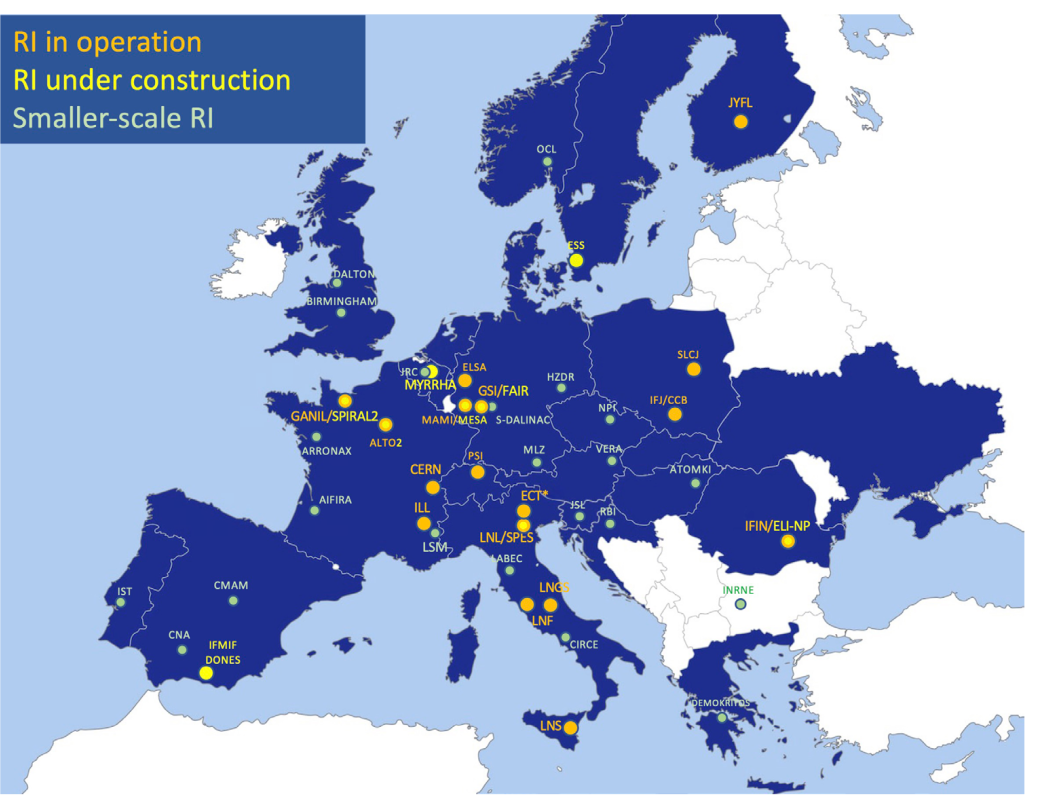
\includegraphics[width=0.6\textwidth]{EuRI.png}
\label{fig:euri}
\caption{Mapa de instalaciones de haces radiactivos en Europa. Extraído del LRP-2024 de NuPECC \cite{nupecc}.}
\end{center}
\end{figure}


A la hora de entender la estructura nuclear, el modelo de capas o modelo de campo medio, por el que Maria Goeppert-Mayer y Johannes Hans Daniel Jensen recibieron el premio Nobel en 1963 \cite{Goe49}, se ha mostrado bastante exitoso en la descripción de las propiedades de núcleos estables. Sin embargo, en su extensión a núcleos inestables se ha encontrado que los números mágicos (número de protones o neutrones que cierran una capa y por tanto crean una configuración particularmente estable) presentan valores distintos a los obtenidos para los núcleos estables y dependientes del ratio entre protones y neutrones de los núcleos, debido, entre otras razones, a la interacción tensorial entre nucleones\cite{Ots20}. 

Otra limitación del modelo de capas, incluso en núcleos estables, es su sobreestimación sistemática de la ocupación de los niveles monoparticulares próximos a la energía de Fermi (el último nivel ocupado). Los números de ocupación de los niveles de valencia obtenidos experimentalmente son sistemáticamente un 60-70\% \cite{Pan97} del valor predicho suponiendo un modelo extremo de campo medio (modelo de partículas independientes, IPM). Esta reducción o \textit{quenching} está asociada a correlaciones entre los nucleones del núcleo, que pueden ser de largo alcance (LRC) \cite{Bar09}, asociadas a excitaciones a energías bajas debidas fenómenos de excitación colectiva y de apareamiento no incluidos en el IPM, o a correlaciones de corto alcance (SRC) \cite{Sub08}, asociada a excitación a energías altas producida por la intensa interacción nuclear entre nucleones muy cercanos. Las estimaciones actuales indican que las LRC provocan una reducción de los números de ocupación del IPM de $10-20\%$, y las SRC una cantidad similar $10-20\%$. Dada la importancia de las correlaciones nucleares no sólo en la descripción de la estructura nuclear, sino en la descripción de la ecuación de estado de la materia nuclear y sus implicaciones astrofísicas (estrellas de neutrones), el LRP-2024 de NuPECC \cite{nupecc} incluye tanto la evolución de las capas nucleares como las correlaciones nucleares entre los puntos de interés en estructura y dinámica nuclear.

Es importante destacar en este punto que ambos estudios (evolución de capas y correlaciones) requieren de la obtención de los números de ocupación (o los relacionados factores espectroscópicos, SF), que experimentalmente se extraen de reacciones nucleares que involucran núcleos exóticos. Por lo tanto, para la obtención de valores fiables es necesaria una descripción precisa de la reacción utilizada, ya que típicamente estos valores se obtienen a partir del cociente entre la sección eficaz experimental y una predicción teórica que supone una ocupación de 1. Un claro ejemplo de la importancia de la descripción de la reacción es el aún no resuelto problema de la dependencia de los factores de \textit{quenching} con la asimetría de isospín:

Como se ha indicado, típicamente, los modelos de estructura sobreestiman la ocupación experimental de los niveles próximos a la energía de Fermi por un porcentaje aproximadamente constante para los núcleos estables. A este cociente entre la ocupación experimental y teórica, o más precisamente, entre la sección eficaz experimental y la teórica (que supone un cierto modelo de estructura para el núcleo y una cierta descripción de la reacción), se le denomina factor de reducción o de \textit{quenching} ($R$). Al extender el estudio de los factores $R$ a núcleos exóticos usando reacciones de arranque de un nucleón a energías intermedias ($\sim$100 MeV por nucleón) con blancos de $^9$Be ó $^{12}$C (reacciones de \textit{knockout}) se encontró una interesante tendencia \cite{Gad08}. Para núcleos con una gran asimetría de isospín (por ejemplo, con muchos neutrones y pocos protones comparado con el núcleo estable de masa similar) al arrancar la partícula más abundante se obtenía un $R$ muy próximo a 1, es decir, que el modelo teórico predecía correctamente la sección eficaz experimental, mientras que al arrancar la partícula menos abundante el factor $R$ era mucho más pequeño, del orden de 0.2-0.4 (frente a 0.6-0.7 para núcleos estables). Medidas experimentales con más núcleos no han hecho más que confirmar esta tendencia \cite{Tos14,Tos21}, y se propuso que esta se debía a un incremento en las SRC para los nucleones en defecto y una reducción para los nucleones en exceso, que se quedaban ``desapareados'' \cite{Jen11}, ya que las SRC favorecen parejas protón-neutrón \cite{Pia06,Sub08}. Esta explicación quedó en entredicho cuando, al realizar un estudio similar con reacciones de transferencia de un nucleón, se encontro que esta tendencia de los factores $R$ desaparecía, encontrándose independencia con la asimetría de isospin \cite{Fla13,Kay13}. Esta diferencia en tendencias queda reflejada en la Figura \ref{fig:gade} (extraída de \cite{Kay22}) y supone un significativo problema para la explicación basada en las correlaciones protón-neutrón, ya que tanto las reacciones de \textit{knockout} como las de transferencia deberían ser sensibles a los mismos números de ocupación, modificados de la misma manera por las correlaciones, por lo que resulta difícil entender cómo dos experimentos a priori equivalentes pueden producir distintos resultados. 

Aquí entra la importancia de la teoría de reacciones nucleares, ya que esta actúa como intermediaria entre los modelos de estructura nuclear y los datos experimentales, por lo que para poder obtener información sobre la estructura nuclear a partir de los datos experimentales es esencial tener bajo control el mecanismo subyacente a la reacción que se está midiendo, sin lo cual, como muestra el ejemplo anterior, los resultados inferidos pueden adolecer de errores fundamentales.

\begin{figure}
\begin{center}
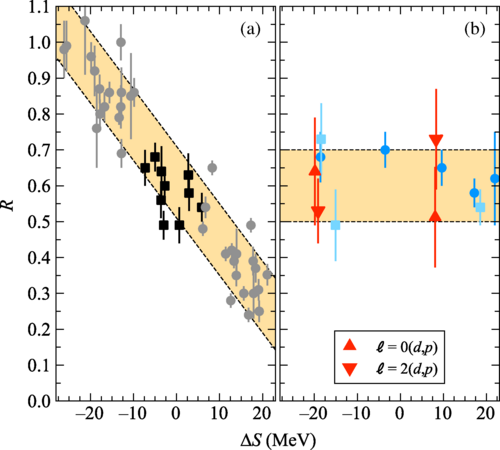
\includegraphics[width=0.6\textwidth]{kay22.png}
\label{fig:gade}
\caption{Dependencia de los factores de reducción $R$ con la asimetría de isospín para reacciones de knockout (izquierda) y reacciones de transferencia (derecha). La asimetría de isospín se cuantifica con la diferencia entre energías de separación de la partícula arrancada y su pareja de isospín $\Delta S=S_{p(n)}-S_{n(p)}$. Figura extraída de \cite{Kay22}}
\end{center}
\end{figure}

El desarrollo de blancos de hidrógeno de alta precisión \cite{Obe14,Pan16,Liu23} ha permitido la utilización de reacciones $(p,pN)$ sobre núcleos exóticos. Estas reacciones, muy populares en los años 60 y 70 \cite{Jac66}, consisten en la colisión de un haz de protones sobre un blanco del núcleo de interés, tras la cual el protón incidente y un nucleón arrancado del núcleo blanco son emitidos formando un ángulo próximo a 90$^\circ$ entre sí. El núcleo residual, con un nucleón menos, también es detectado. La dificultad que aparece para núcleos radiactivos es la imposibilidad de construir un blanco con ellos debido a su corta vida, por lo que las reacciones medidas en los 60 y 70, con haces de protones, no son posibles. Sin embargo, si un blanco de protones es accesible, el experimento puede realizarse en cinemática inversa, usando un haz del núcleo de interés colisionando sobre el blanco de protones. Este tipo de reacciones presentan un mecanismo de colisión muy sencillo, y de hecho, se denominan \textit{quasi-free}, porque el proceso de colisión entre el protón incidente y el nucleón arrancado es análogo a una colisión libre entre ambos, de ahí el ángulo próximo a 90$^\circ$. Este mecanismo de reacción sencillo, unido a la clara señal experimental (nucleones a 90$^\circ$) incitó a la aplicación de las reacciones $(p,pN)$ a numerosos núcleos exóticos durante la década de 2010 \cite{Ata18,Kaw18,Pau19,Hol19} y en particular se abordó el problema de la dependencia de los factores de reducción con la asimetría de isospín, encontrándose poca dependencia con la asimetría \cite{Ata18,Kaw18}, en mejor acuerdo con los resultados encontrados en las reacciones de transferencia, y por lo tanto, dando un menor efecto de las SRC de lo que se podía intuir en base a las reacciones de \textit{knockout}. En el LRP-2024 se indica que ``El uso de reacciones $(p, pN)$ se ha convertido en una herramienta muy versatil, que en el futuro cercano continuará siendo una sonda experimental clave'', destacando la importancia actual de este tipo de reacciones, con instalaciones como $R^3B$, en Europa \cite{r3b24} u ONOKORO \cite{onokoro}, en Japón, optimizadas para realizarlas.

El acceso a blancos de hidrógeno también ha propiciado el interés por las reacciones de arranque de dos nucleones $(p,p2N)$, en particular las reacciones de arranque de dos protones $(p,3p)$ de núcleos ricos en neutrones, lo cual permite producir especies muy exóticas, con gran asimetría entre el número de protones y neutrones, en estados excitados no accesibles con otros mecanismos de reacción \cite{Tan19}. Además, las reacciones $(p,3p)$ sobre núcleos exóticos son una prometedora sonda para estudiar las correlaciones nucleón-nucleón, dado que se han empleado exitosamente con este objetivo en núcleos estables \cite{Pia06}. Por esto, las instalaciones de proyectos como ONOKORO \cite{onokoro} y FAIR/R$^3$B \cite{r3b24,nupecc} están siendo diseñadas para permitir el análisis de reacciones $(p,3p)$, reacciones de interés actual en la comunidad de física nuclear, para las que hasta muy recientemente no existía una descripción teórica que permitiera el cálculo de secciones eficaces, la cual ha sido desarrollada por el candidato \cite{p3p}.

La relación entre teoría de estructura nuclear y teoría de reacciones nucleares, ejemplificada en los párrafos anteriores en el caso de la dependencia de los factores de reducción con la asimetría de isospín es uno de los puntos de interés en la comunidad de física nuclear teórica, en particular, las incertidumbres producidas por la posible inconsistencia entre los modelos de estructura y reacciones empleados. De hecho, de las recomendaciones hechas en la sección de estructura y dinámica nuclear del LRP-2024 \cite{nupecc}, la única concerniente a los desarrollos teóricos insta al desarrollo de una teoría consistente de estructura nuclear y de reacciones nucleares. Esto constituye un desafío importante, ya que los modelos de muchos cuerpos empleados en estructura nuclear presentan serias dificultades al tratar con las numerosas configuraciones (o canales) que se hacen disponibles en los sistemas no ligados correspondientes a las reacciones nucleares. Una vía prometedora para esta unificación es el desarrollo de potenciales ópticos obtenidos de primeros principios \cite{Idi19} o utilizando modelos dispersivos \cite{Cha07}, que correlacionan las propiedades de los estados de energías positivas, correspondientes a dispersión entre núcleos (reacciones nucleares) con los estados de energías negativas, correspondientes a estados ligados (estructura nuclear). Estos potenciales ópticos son luego utlizados en descripciones de reacción para obtener los observables experimentales, obteniendo así una descripción consistente de estructura y reacciones. Una dificultad en este desarrollo es el hecho de que la mayoría de teorías de reacciones y códigos que las implementan están basados en potenciales ópticos fenomenológicos obtenidos en base al ajuste de datos experimentales, que presentan propiedades distintas a los potenciales obtenidos en base a modelos dispersivos o de primeros prinicipios. En particular, los potenciales fenomenológicos son típicamente locales e independientes de la energía, mientras que los potenciales ópticos de primeros principios son no locales y dependientes de la energía (como corresponde a un potencial óptico ``exacto'' de acuerdo a la teoría de Feshbach \cite{Fes58}). Es por lo tanto esencial adaptar las teorías (y códigos) de reacciones existentes para que puedan incorporar potenciales no locales y dependientes de la energía para obtener el objetivo de una teoría consistente de estructura y reacciones. Este es un punto de desarrollo actualmente activo en la comunidad de teoría de reacciones nucleares \cite{Tim13,Bai16,Tit16,Lov17,Heb21}.

Dentro de este contexto se desarrolla la carrera del investigador candidato y se proponen las líneas de investigación que el candidato desarrollaría tras la obtención de la plaza en este concurso.

\textbf{Antecedentes y experiencia previa}

El candidato ha centrado su investigación en la teoría de reacciones directas con particular interés en reacciones de arranque de una o dos partículas.

Debido a las varias campañas experimentales centradas en experimentos a energías intermedias con blancos de protones \cite{r3b07,Kaw18}, indicadas en la sección anterior, el candidato centró su tesis doctoral en el estudio de reacciones de arranque de un nucleón $(p,pN)$, implementando para ello un formalismo basado en el cálculo de transferencia al continuo (TC) para regímenes relativistas \cite{Mor15}. Este formalismo es distinto y complementario al fórmalismo de aproximación de impulso con ondas distorsionadas (DWIA) \cite{Jac66} utilizado tradicionalmente en la descripción de las reacciones $(p,pN)$, lo cual es particularmente relevante a la hora de validar el mecanismo de reacción, puesto que si dos modelos con aproximaciones distintas presentan resultados similares es esperable que las aproximaciones de los modelos sean adecuadas para la descripción del proceso físico. El candidato realizó comparaciones con cálculos utilizando DWIA en una estancia de colaboración en el centro RCNP de Osaka, Japón, bajo la supervisión del profesor K.~Ogata \cite{benchmarkdwia} y con cálculos utilizando el formalismo Faddeev/AGS \cite{Fad60, Alt67} en colaboración con el profesor A.~Deltuva \cite{benchmarkfaddeev}, encontrando en ambos casos acuerdos satisfactorios que validan su formalismo. La aplicación de los cálculos TC a las medidas de reacciones $(p,pN)$ sobre isótopos de nitrógeno y oxígeno revelaron una relativa independencia de los factores de reducción con la asimetría de isospín \cite{ppn}, extendiendo y validando otros análisis previos basados en DWIA \cite{Ata18}. El candidato ha participado en el análisis posterior de otros experimentos $(p,pN)$ \cite{thomas,49cl,49ar}.

Además, el candidato colaboró con el doctor J.~Casal, del departamento de FAMN, para extender los estudios $(p,pN)$ a sistemas de tres cuerpos, en particular el $^{11}$Li, encontrando un buen acuerdo con datos experimentales tanto para la reacción $(p,pn)$ a energías altas \cite{11lippn} como para la reacción de transferencia $(p,d)$ a energías bajas \cite{11lipd}, usando un modelo para el $^{10}$Li (núcleo no ligado residual en ambas reacción) que también describía satisfactoriamente la reacción $^9$Li$(d,p)^{10}$Li \cite{9lidp}. El desarrollo de la extensión de los cálculos $(p,pN)$ a núcleos de tres cuerpos permitió al candidato establecer una fructífera colaboración con el grupo experimental de la doctora A.~Corsi de CEA/Université Paris-Saclay, Francia, centrada en el estudio de otros núcleos de tres cuerpos, como el $^{14}$Be \cite{14be,openingangle}.

Dada la discrepancia entre las tendencias de los factores de reducción de las reacciones de \textit{knockout} por un lado y las de transferencia y $(p,pN)$ por otro lado, el candidato ha explorado posibles puntos de mejora de la descripción de las descripciones de \textit{knockout} que permitan corregir esta diferencia, centrándose en los posibles efectos de pérdida de sección eficaz debido a la interacción del nucleón arrancado y el núcleo residual formado, que puede llevar a la ruptura del último.  El candidato, junto con sus colaboradores del departamento de FAMN, los profesores A.M.~Moro y J.~Gómez Camacho, ha sido capaz de desarrollar formalismos que incluyen estos efectos \cite{complexcdcc,quenching}, encontrando en unos primeros resultados, una significativa reducción de la dependencia de los factores de reducción con la asimetría de isospín, mejorando de manera importante el acuerdo entre el comportamiento para las reacciones de \textit{knockout} y las de transferencia y $(p,pN)$ al tener en cuenta estos efectos.

Durante su contrato postdoctoral en la Technische Universität Darmstadt, el candidato colaboró con el grupo experimental local, liderado por el profesor A.~Obertelli, en el estudio de las reacciones $(p,3p)$ en núcleos ricos en neutrones de masa intermedia a energías intermedias. Mediante el uso de modelos cinemáticos, el candidato demostró que las distribuciones angulares de los protones salientes en estas reacciones eran mayoritariamente compatibles con parejas de protones poco correlacionadas, o correlacionadas a través de LRC, por lo que, salvo selecciones cinemáticas muy estrictas, estos protones no parecen adecuados para explorar las SRC \cite{axel}. Sin embargo, siguen siendo buenos candidatos para la producción de núcleos exóticos, por lo que el candidato ha desarrollado recientemente el primer formalismo capaz de realizar predicciones cuantitativas de las secciones eficaces a distintos estados del núcleo residual \cite{p3p}, cálculos que está utilizando actualmente en el análisis de datos experimentales para reacciones $(p,3p)$ en colaboración con el grupo del profesor Obertelli.

Durante el periodo predoctoral, el candidato también ha mostrado interés en reacciones a baja energía y la extensión de sus descripciones para considerar mecanismos y efectos no contemplados en los formalismos clásicos. Entre estas extensiones se incluyen la inclusión de efectos de excitación del \textit{core} en reacciones de transferencia (su trabajo de máster \cite{transferx}) o la inclusión de excitaciones del blanco en procesos de ruptura del proyectil \cite{texc,texctransfer}, trabajo que ha derivado en colaboraciones experimentales \cite{vinicius}. Especial mención debe hacerse al estudio de la inclusión de no localidad que el candidato ha realizado en colaboración con la doctora N.K.~Timofeyuk en sus estancias pre- y postdoctorales en la Universidad de Surrey, Reino Unido, donde el candidato desarrolló extensiones del método de canales acoplados con discretización del continuo para la inclusión de no localidad en reacciones con efectos de ruptura del proyectil \cite{Tim18,Tim19,Fro23} y otras extensiones como la inclusión de fuerzas de tres cuerpos \cite{3nf}. 

Además, el candidato ha contribuido de manera activa en el desarrollo del código de estructura y reacciones nucleares de código abierto del grupo de teoría de reacciones nucleares de la Universidad de Sevilla, THOx \cite{thox}, en colaboración con los profesores del Departamento de Física Atómica, Molecular y Nuclear A.M.~Moro, J.~Casal y J.A.~Lay. En la versión disponible actualmente, el candidato ha implementado la posibilidad de calcular reacciones con ruptura del proyectil y excitación simultánea de estados colectivos del blanco \cite{texc} y el cálculo de secciones eficaces de fotodisociación y captura radiativas para transiciones eléctricas $E\lambda$. También ha paralelizado los pesados cálculos de secciones eficaces de tres cuerpos para reacciones de ruptura (secciones diferenciales angulares en función del ángulo y la energía de emisión de los fragmentos de ruptura).


\textbf{Líneas de investigación}

A continuación, se describe la propuesta investigadora del candidato. La propuesta
está dividida en cuatro líneas de investigación (L1-L4) alineadas con los antecedentes previamente descritos, la experiencia del candidato y el perfil investigador de la plaza.

\underline{L1: Reacciones de arranque de una partícula: reacciones $(p,pN)$, \textit{knockout} y} \newline \underline{transferencia}

Dado el poder espectroscópico de las reacciones de arranque de una partícula, es esperable que dichas reacciones sigan siendo un importante foco de interés experimental en el futuro, ya que permiten el estudio de problemas de importante interés para la comunidad de física nuclear. Por lo tanto, el candidato propone la continuación de su exploración de los efectos de destrucción del core en reacciones de \textit{knockout} de una partícula \cite{quenching}, extendiendo su estudio a más núcleos para los que existen medidas experimentales \cite{Tos21} e intentando cuantificar las incertidumbres provocadas por el uso de potenciales ópticos mediante el uso de varias prescripciones realistas. Dado que el método utilizado hasta la fecha es un método semiclásico \cite{quenching}, el desarrollo de expresiones completamente cuánticas sería valioso para evaluar los sesgos provocados por la aproximación semiclásica. Estos proyectos tendrán el apoyo de los co-autores del departamento de FAMN de los estudios previos: J.~Gómez Camacho y A.M.~Moro.

Es esperable que en el futuro cercano se realicen numerosas reacciones en cinemática inversa con blancos de protones tanto en las instalaciones GSI/FAIR en Alemania y RIKEN en Japón, esta última dentro del proyecto ONOKORO\cite{r3b24,onokoro}. En estos experimentos, las reacciones de arranque de nucleones $(p,pN)$ podrán ser fácilmente medidas gracias a su sección eficaz relativamente elevada y a su clara señal experimental. La experiencia del candidato en reacciones $(p,pN)$, foco de su tesis doctoral, será muy relevante en el estudio de estas reacciones. Dado que los núcleos de interés corresponden a un rango de masas medio $A\sim 50-200$, los cálculos de la estructura de dichos núcleos pueden resultar dificultosos, para lo cual el candidato buscará el apoyo de T.R.~Rodríguez Frutos, miembro del departamento de FAMN y experto en estructura nuclear.

Para núcleos más pesados es necesario que los cálculos se extiendan a valores del momento angular total mayores $J\sim 100$, para los cuales los cálculos de Transferencia al Continuo empleados se vuelven más inestables debido al incremento de la barrera centrífuga. Por ello, el candidato explorará métodos para reducir esta inestabilidad, tales como la implementación de un cálculo eikonal para valores grandes de $J$ o el desarrollo de un método de extrapolación de las matrices $S$ usando fórmulas asintóticas con una posible combinación con técnicas de IA. El éxito de estos métodos tendría una extensión natural a otros tipos de reacciones, como transferencia o breakup coulombiano, que también sufren de estas inestabilidades.

\underline{L2: Reacciones de arranque de dos partículas: reacciones $(p,3p)$}

Como se ha indicado en los antecedentes y en la línea de investigación anterior, el desarrollo de blancos de hidrógeno de alta resolución ha incrementado el interés por las reacciones con protones, lo que, unido al interés de la comunidad por las correlaciones entre nucleones, hace que las reacciones de arranque de dos protones $(p,3p)$ sean un elemento importante de futuros programas experimentales en instalaciones como RIKEN, dentro del proyecto ONOKORO\cite{onokoro}.

Dado que el candidato desarrolló durante su estancia postdoctoral en la Technische Universität Darmstadt un formalismo semiclásico para el cálculo de secciones eficaces de estas reacciones, se encuentra en una situación perfecta para dar apoyo teórico a los grupos que van a realizar estos experimentos. De hecho, en la actualidad se encuentra en una colaboración con el grupo experimental de la TU Darmstadt con quien realizó la estancia (C.~Xanthopoulos, M.~Enciu y A.~Obertelli) para el análisis de varios experimentos $(p,3p)$ en núcleos en el rango de masas del $^{52}$Ca. Además, ha colaborado en propuestas para los experimentos $^{70}$Zn$(p,3p)^{68}$Ni y $^{10}$Be$(p,3p)^8$He con H.~Liu de la Universidad Normal de Pekín y Y.~Sun de la Universidad de Beihang.

Aparte de estas colaboraciones, el candidato pretende extender el estudio de las reacciones $(p,3p)$, para las cuales ahora sólo puede calcular secciones eficaces totales para cada estado del núcleo residual. El candidato pretende desarrollar un formalismo semiclásico para el cálculo de distribuciones de momentos del núcleo residual, con aplicaciones espectroscópicas, además de desarrollar un modelo puramente cuántico para la descripción de estas reacciones, cuya aproximación semiclásica puede introducir incertidumbres en los resultados. Como en el caso de las reacciones de arranque de un nucleón, el avance a núcleos más pesados introduce una mayor complejidad en el cálculo de estructura nuclear necesario para la descripción de estas reacciones, por lo que el candidato buscará una vez más el apoyo del profesor T.R.~Rodríguez Frutos del departamento de FAMN.

El candidato también explorará el estudio comparativo de las reacciones de arranque de dos protones $(p,3p)$ con las reacciones de transferencia de dos protones, como $(n,^3$He$)$, dada la amplia historia de las reacciones de transferencia de dos partículas en el estudio de correlaciones entre nucleones. Para ello, el candidato buscará el apoyo del profesor del departamento J.A.~Lay, que posee una amplia experiencia en el estudio de reacciones de transferencia de dos nucleones.

\underline{L3: Desarrollo de la teoría de reacciones a bajas energías}

Las reacciones $(p,pN)$ y $(p,3p)$ se miden a energías intermedias ($\sim$100-500 MeV/A) para maximizar el recorrido libre medio de los núcleones dentro del núcleo y así obtener una reacción ``limpia'' de un solo paso. Sin embargo, el campo de experiencia tradicional del grupo de teoría de reacciones del departamento de FAMN  son reacciones a energías más bajas y de hecho el candidato también posee experiencia en reacciones a estas energías.

Por ello, el candidato también pretende desarrollar extensiones y mejoras en las teorías utilizadas para la descripción de reacciones a energías más bajas. Una de estas mejoras es la inclusión de la excitación del \textit{core} en reacciones con sistemas de tres cuerpos, punto en el que colabora en la actualidad con el miembro del departamento de FAMN J.~Casal, experto en modelos de tres cuerpos.

Otro punto de desarrollo en la teoría de reacciones a energías bajas es la inclusión de potenciales no locales, punto en el que el candidato ha colaborado con la doctora N.K.~Timofeyuk de la Universidad de Surrey, Reino Unido, previamiente \cite{Tim18,Tim19,Fro23}. Dado que la inclusión de la no localidad en teorías estándar de reacción es fundamental para el uso de potenciales \textit{ab initio} obtenidos a partir de primeros princios y que  el uso de estos potenciales perimite una mayor consistencia entre las teorías de estructura y reacciones nucleares, este es un desarrollo importante, para lo cual el candidato pretende continuar la colaboración con la doctora N.K.~Timofeyuk en el estudio de la no localidad.

Particularmente interesante sería la aplicación de potenciales no locales a las reacciones de ruptura no elástica (NEB) con producción de partículas $\alpha$, que presentan unas sobreestimaciones significativas en la comparación entre teoría y experimento, lo cual requiere la inclusión de no localidad en el formalismo Ichimura-Austern-Vincent (IAV), cuya implementación fue realizada por el doctor J.~Lei de la Universidad de Tongji, China, y el profesor del departamento de FAMN A.M.~Moro \cite{iav}. El resultado de una colaboración en este punto con ellos podría ser relevante para el estudio de la clusterización $\alpha$ en núcleos ligeros y medianos.

\underline{L4: Apoyo teórico a la comunidad experimental:  desarrollo de herramientas de acceso}\newline \underline{abierto}

Dada la estrecha relación entre la teoría de reacciones nucleares y los observables experimentales, es fundamental para un físico especializado en teoría de reacciones mantener una estrecha colaboración con los grupos experimentales y servirles de apoyo tanto en la propuesta de medidas experimentales como en el posterior análisis de los experimentos. Como se ha indicado en la sección de antecedentes, el candidato ha participado en numerosas colaboraciones experimentales y actualmente se halla involucrado en colaboraciones con los grupos de R.~Smith, H.~Liu y Y.~Sun para las medidas experimentales de las reacciones $^7$Be$(d, p)^8$Be$^*$, $^{70}$Zn$(p,3p)^{68}$Ni y $^{10}$Be$(p,3p)^8$He respectivamente.

Dado el compromiso del candidato con la ciencia abierta, el candidato también pretende continuar su desarrollo del código abierto THOx. Futuras mejoras del código que el candidato pretende desarrollar son el cálculo de canales acoplados con potenciales complejos que den cuenta de la posible ruptura del core debido a su interacción con la partícula de valencia \cite{complexcdcc} y el cálculo de secciones eficaces en función del ángulo interno protón-neutron para reacciones de ruptura del deuterón, para las cuales ya ha desarrollado implementaciones que deben ser incorporadas a la versión pública del código. Otros puntos de mejora que el candidato ha iniciado pero que aún no cuentan con implementación son el cálculo exacto de estados ligados dentro del modelo de potencial y el cálculo de la probabilidad de excitación magnética B(M$\lambda$) y las secciones eficaces de fotodisociación y captura radiativa asociadas.

Dentro de este punto, también cabe mencionar la participación del candidato en el grupo teórico (Theo4Exp) del proyecto europeo EUROLABS \cite{eurolabs} y su compromiso con el acceso global a cálculos de reacciones nucleares de última generación, mencionado en la sección de antecedentes. Además de su participación en la difusión y soporte de este proyecto, el candidato pretende implementar mejoras en el actual dispositivo online, guíado principalmente por las sugerencias de los usuarios en el reciente taller en el que participó en Julio de 2025 \cite{Workshop_Trento_25}. Estas mejoras incluirían: la posibilidad de seleccionar potenciales globales en los cálculos de reacciones de transferencia, la implementación de más parametrizaciones en la lista de potenciales globales, la introducción de ajuste de mínimos cuadrados para la obtención de potenciales ópticos a partir de datos experimentales o el cálculo de secciones eficaces de captura radiativa. En estos puntos el candidato cuenta con el apoyo de los otros miembros del departamento de FAMN que participan en este proyecto: M.~Rodríguez Gallardo (IP), A.M. Moro, J.A.~Lay y C.T.~Muñoz.

\subsubsection{Financiación e infraestructura}

Las líneas de investigación propuestas se encuentran dentro de los objetivos del proyecto nacional PID2023-146401NB-I00, vigente hasta 2027, mientras que la colaboración en el proyecto EUROLABS cuenta con financiación del proyecto europeo 4598/1176, vigente hasta 2026. Por otra parte, se espera concurrir a próximas convocatorias de los proyectos asociados a la estrategia de I+D+I de Andalucía (EIDIA 2021-2027).

Dado el carácter preeminentemente teórico de las líneas de investigación propuestas, la infraestuctura requerida principalmente consiste en servidores de computación capaces de realizar los cálculos teóricos necesarios. El Departamento de FAMN cuenta con un modesto servidor de computación interno con el que realizar la mayoría de los cálculos. Los proyectos en activo incluyen presupuesto para equipos de computación con objetivo de mejorar los equipos del Departamento de FAMN, así como para gastos de viajes y participación en congresos. 

En caso de requerir más capacidad de computación, el candidato tiene acceso a los servicios de computación del CICA (Centro Informático
Científico de Andalucía), así como al servicio de supercomputación PROTEUS, que pueden ser de utilidad al afrontar cálculos pesados o extensivos.

Con el objetivo de financiar la formación de investigadores jóvenes a través de la dirección de trabajos de tesis, el candidato planteará su participación en futuras convocatorias de proyectos autonómicos o estatales como Investigador Principal en solicitudes individuales o junto con el grupo de investigación FQM-160.

%\addbibresource{refs_proj.bib}

\bibliographystyle{unsrt2authabbrvpp} %MGR: ChatGPT me ha sujerido este estilo, parece que con este el orden sale bien pero revisalo
\bibliography{refs_proj}




\end{document}






